\chapter{THE EFFECT OF HIGH LASER POWER ON INTERFEROMETER ALIGNMENT}
\label{ch:eigenmodes}

% \section{Dynamic response of coupled pendula}


The torque induced by radiation pressure, as introduced in
Sec. \ref{sec:rp_intro}, couples the angular motion of the suspended
mirrors, complicating the plant for which controls must be
designed. The derivation of the angular response of the mirrors to
external torque in the presence of radiation pressure is presented in
several publications, but I provide my own derivation here for
completeness. Radiation pressure torque is, after all, the foundation
for this work's investigation of high power effects in the angular
sensing and control. We derive a set of eigenfunctions that
diagonalize the linear cavity's response to radiation pressure and
describe the mirrors' equations of motion in this new eigenbasis. We
show that the torque to angle transfer functions of the new eigenmodes
are modified such that one mode is statically unstable at Enhanced
LIGO powers.

% \textcolor{blue}{this needs re-writing} Namely, radiation pressure
% torque has the effect of breaking the symmetry of the equations of
% motion of each of the mirrors. Since Enhanced LIGO embarks on the path
% of increasing the laser power, examining the effect of radiation
% pressure torque in detail is warranted. 





\section{The Radiation Pressure Angular Spring}
The geometric axis of a cavity formed by two spherical mirrors is
dictated by the line joining the two centers of curvature. Only if the
mirrors are pointed directly at one another will the cavity geometric
axis pass through the centers of the mirrors. Should a laser beam
resonate in the cavity, it will do so along this geometric axis. Thus,
if the mirrors are tilted away from one another, the beam spot on each
mirror will not be centered. The relationship between the positions of
the beams on the mirrors relative to center, $x_i$, and the angles of
the mirrors, $\theta_i$, is given by:
\begin{equation}
\left\llbracket \begin{array}{c}
x_1\\
x_2 \end{array} \right\rrbracket = \frac{L}{1-g_1 g_2}
\left\llbracket \begin{array}{cc}
g_2 & 1\\
1 & g_1\end{array} \right\rrbracket
\left\llbracket \begin{array}{c}
\theta_1\\
\theta_2 \end{array} \right\rrbracket .
\label{eq:x}
\end{equation}
The $g$-factor is defined as $g_i=1-R_i/L$ where $R_i$ is the mirror
radius of curvature, and $L$ is the length of the cavity. The
$g$-factor is $0.73$ ($0.71$) for the LLO (LHO) ITM and $0.54$
($0.45$) for the LLO (LHO) ETM.

We saw in the previous chapter that the radiation pressure torque on a
mirror depends on the position of the beam on the mirror, $\tau_{rp} =
2 P x / c$ (Eq. \ref{eq:tau_rp}). Based on Eq. \ref{eq:x} the
radiation pressure torque on a mirror that is part of a
Fabry-P\'{e}rot cavity is therefore dependent on the angle of both the
mirror of interest and the second mirror forming the cavity:
\begin{equation}
\left\llbracket \begin{array}{c}
\tau_{rp,1}\\
\tau_{rp,2} \end{array} \right\rrbracket = \frac{2 P L}{c (1-g_1 g_2)}
\left\llbracket \begin{array}{cc}
g_2 & 1\\
1 & g_1\end{array} \right\rrbracket
\left\llbracket \begin{array}{c}
\theta_1\\
\theta_2 \end{array} \right\rrbracket.
\end{equation}
This is more succinctly expressed as
\begin{equation}
\vec{\tau}_{rp} = -\mathbf{K_{rp}} \vec{\theta},
\label{eq:rpspring}
\end{equation}
where $\mathbf{K_{rp}}$ is the \emph{torsional stiffness
  matrix}. Equation \ref{eq:rpspring} is the expression that describes
the radiation pressure angular spring.




\subsection{Diagonalizing the Modified Equations of Motion}
\label{sec:eigenbasis}
The radiation pressure spring modifies the pendulum angular equation
of motion and therefore the torque to angle transfer function
through the addition of an angle-dependent torque term. Re-writing
Eq. \ref{eq:eqmotion} in matrix form and with the radiation pressure
spring term, the two equations that describe the motion of two mirrors
forming a Fabry-P\'{e}rot cavity is: 
\begin{equation}
\mathbf{I} \ddot{\vec{\theta}} 
+ {\bm \gamma} \dot{\vec{\theta}} 
+ \mathbf{\kappa_p} \vec{\theta}
- \frac{2 P L}{c (1-g_1 g_2)}
\left\llbracket \begin{array}{cc}
g_2 & 1\\
1 & g_1\end{array} \right\rrbracket \vec{\theta} 
= \vec{\tau}_{ext}.
\label{eq:motion_rp}
\end{equation}
$\mathbf{I}$, $\gamma$, and $\kappa_p$ are $2 \times 2$ diagonal
matrices and $\vec{\theta}$ and $\vec{\tau}_{ext}$ are $2 \times 1$
vectors as in the previous section. Due to the non-diagonal matrix in
Eq. \ref{eq:motion_rp}, the motions of each of the mirrors forming the
cavity are tied to one another. The natural way to work with such a
system is to rotate the coupled equations into a new basis. The
resulting de-coupled equations of motion will described specific
combinations of mirror tilts instead of the tilt of an individual mirror. Vectors in
the rotated basis are written with primes.

In order to decouple the two equations of Eq. \ref{eq:motion_rp}, we
need to diagonalize $\mathbf{K_{rp}}$. The subscripts $a$ and $b$ are
used to denote the elements of the diagonalized basis, to contrast the
$1$ and $2$ which denote the mirror basis. Ignoring the constants of
matrix $\mathbf{K_{rp}}$, its eigenvalues are
\begin{align}
\lambda_a &= \frac{g_1 + g_2 + \sqrt{(g_1 - g_2)^2 + 4}}{2} \\
\lambda_b &= \frac{g_1 + g_2 - \sqrt{(g_1 - g_2)^2 + 4}}{2} 
\label{eq:eigenvalues}
\end{align}
and its eigenvectors are
\begin{align}
\vec{v}_a &= \left\llbracket \begin{array}{c} 
1 \\
\frac{g_1 - g_2 + \sqrt{(g_1 - g_2)^2 + 4}} {2} \end{array} \right\rrbracket\\
\vec{v}_b &= \left\llbracket \begin{array}{c}
\frac{ -g_1 + g_2 - \sqrt{(g_1 - g_2)^2 + 4}}{2} \label{eq:eigenvectors}\\
1 \end{array} \right\rrbracket .
\end{align}
Therefore, the matrix 
\begin{equation}
\mathbf{S} = \left\llbracket \begin{array}{cc} 
\vec{v}_a & \vec{v}_b \end{array} \right\rrbracket =
\left\llbracket \begin{array}{cc}
 1 & \frac{-g_1 + g_2 - \sqrt{(g_1 - g_2)^2 + 4}} {2}\\
 \frac{g_1 - g_2 + \sqrt{(g_1 - g_2)^2 + 4}} {2} & 1\end{array} \right\rrbracket
\label{eq:S}
\end{equation}
diagonalizes $\mathbf{K_{rp}}$ such that 
\begin{equation}
\mathbf{S^{-1} K_{rp} S} = \mathbf{D} = \left\llbracket \begin{array}{cc} 
\lambda_a & 0 \\
0 & \lambda_b \end{array} \right\rrbracket = \left\llbracket \begin{array}{cc}
 \frac{g_1 + g_2 + \sqrt{(g_1 - g_2)^2 + 4}}{2}  & 0\\
 0 & \frac{g_1 + g_2 - \sqrt{(g_1 - g_2)^2 + 4}}{2}\end{array}
\right\rrbracket .
\label{eq:diag}
\end{equation}
The matrix of eigenvectors, $\mathbf{S}$, is the basis transformation
matrix. It serves to define the torque and angle vectors in the new
basis. For example,
\begin{equation}
\vec{\theta}^\prime = \left\llbracket \begin{array}{c}
\theta_a\\
\theta_b \end{array} \right\rrbracket = \mathbf{S^{-1}}
\left\llbracket \begin{array}{c}
\theta_1\\
\theta_2 \end{array} \right\rrbracket
= \mathbf{S^{-1}} \vec{\theta}.
\end{equation}

Rearranging Eq. \ref{eq:diag} to the form $\mathbf{K_{rp}} =
\mathbf{S D S^{-1}}$ and substituting it into Eq. \ref{eq:motion_rp},
we have:
\begin{equation}
\mathbf{I} \ddot{\vec{\theta}} 
+ {\bm \gamma} \dot{\vec{\theta}} 
+ \mathbf{\kappa_p} \vec{\theta}
- \frac{2 P L}{c (1-g_1 g_2)} \mathbf{S D S^{-1}} \vec{\theta} 
= \vec{\tau}_{ext} 
\end{equation}
Multiplying on the left by $\mathbf{S^{-1}}$, taking advantage of the
diagonal $\mathbf{I}$, $\gamma$, and $\kappa_p$ matrices, and using
$\mathbf{S^{-1}}$ to change the basis of each of the vectors, the
de-coupled equations of motion are:
\begin{equation}
\mathbf{I} \ddot{\vec{\theta}}^\prime 
+ {\bm \gamma} \dot{\vec{\theta}}^\prime 
+ \mathbf{\kappa_p} \vec{\theta}^\prime
- \frac{2 P L}{c (1-g_1 g_2)}
\left\llbracket \begin{array}{cc}
\lambda_a & 0\\
0 & \lambda_b \end{array} \right\rrbracket \vec{\theta}^\prime 
= \vec{\tau}_{ext}^\prime.
\label{eq:rp_eqmotion}
\end{equation}
The radiation pressure torsion constant, $\kappa_{rp}$, is 
\begin{equation}
\kappa_{rp} = - \frac{2 P L}{c (1-g_1 g_2)} \lambda
\end{equation}
where $\lambda = \lambda_a$ or $\lambda_b$, depending on the mode in
question. 

The angular motion of the Fabry-P\'{e}rot cavity is no longer
described by the motions of its individual mirrors. Due to radiation
pressure, the cavity is treated as a unit and the two orthogonal modes
of angular motion are combinations of the two mirrors' angles. The
eigenvectors $\vec{v}_a$ and $\vec{v}_b$ describe these two sets of
orthogonal mirror tilts, and the eigenvalues $\lambda_a$ and
$\lambda_b$ (along with their common constants) quantify the magnitude
of the radiation pressure torsional spring constant for each of the
modes. While the equations of motion had been identical for each of
the individual mirrors, the decoupled equations in the presence of
radiation pressure breaks that symmetry.


\begin{table}
\centering
\caption[Geometric parameters of the LIGO arm cavity
  eigenmodes]{Geometric parameters of the LIGO arm cavity
  eigenmodes. $x_i$ are the beam locations on the mirrors relative
  to center, $a$ is the cavity axis displacement at the waist, and
  $\alpha$ is the cavity axis angle with respect to a line joining the
  centers of the mirrors. Differences between LLO and LHO arise from the
  mirrors at each site having different radii of curvature. Quantities
  are expressed as a function of the amount of tilt in a particular mode.}
\begin{tabular}{l l r@{}l l l l}
\hline
& & \multicolumn{2}{l}{LLO} & LLO & LHO & LHO \\
cavity parameter & unit & \multicolumn{2}{l}{$\vec{v}_a$ mode} & $\vec{v}_b$ mode & $\vec{v}_a$ mode & $\vec{v}_b$ mode \\
\hline
$|x_1|$ & mm/urad & 9&.88 & 2.44 & 8.20 & 2.51\\
$|x_2|$ & mm/urad & 10&.84 & 2.22 & 9.35 & 2.20\\
$|a|$ & mm/urad & 10&.17 & 1.01 & 8.48 & 1.34 \\
$|\alpha|$ & urad/urad & 0&.24 & 1.17 & 0.29 & 1.18 \\
\hline
\end{tabular}
\label{table:cav_geometric}
\end{table}


Table \ref{table:cav_geometric} outlines the characteristics of these
two eigenmodes for the specific geometry of the LIGO arm cavities. The
amount of beam displacement on each mirror is given as a function of
the amount of tilt in one eigenmode or the other. Furthermore, the
amount of cavity axis displacement $a$ and cavity axis tilt $\alpha$
is also calculated for each eigenmode using the geometric relationship
between a set of mirror tilts and their cavity axis as derived in
Appendix \ref{sec:misaligned_cavity}. Figure \ref{fig:ss} illustrates
a cavity in each of the two eigenmodes when using the parameters from
Table \ref{table:cav_geometric}.


\begin{figure}
\begin{centering}
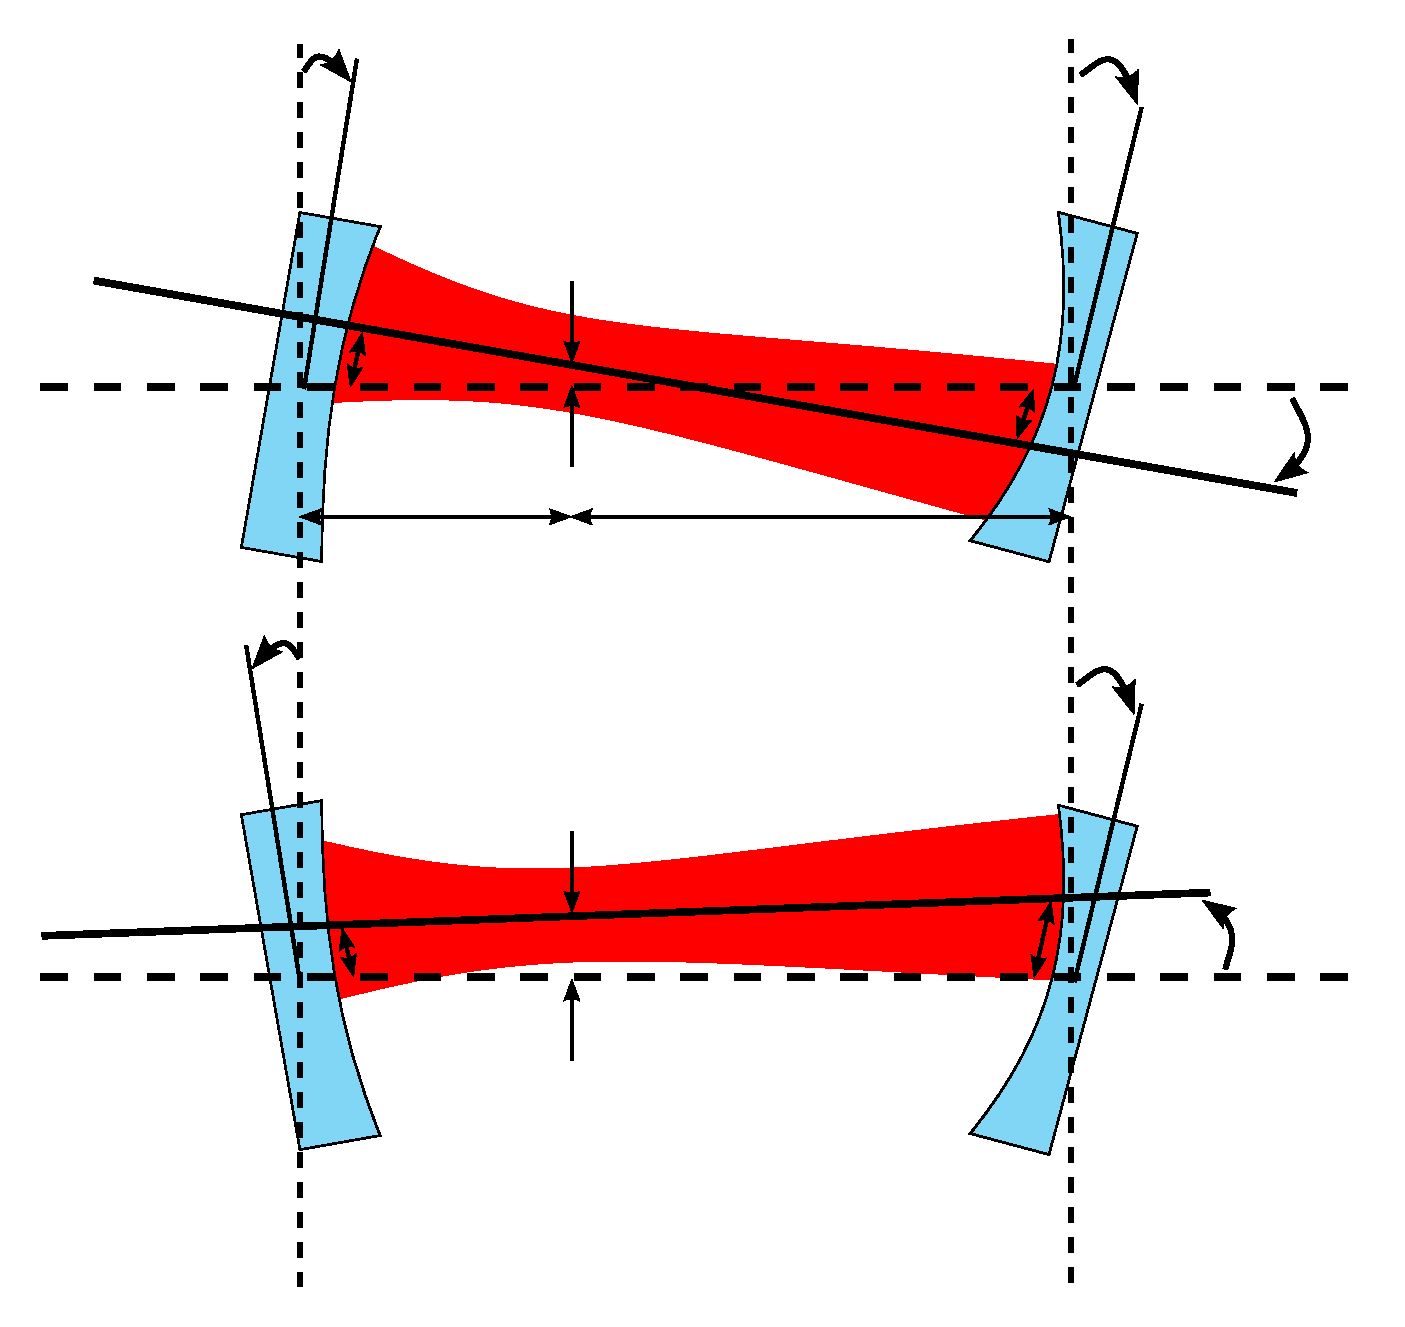
\includegraphics[width=0.7\columnwidth]{figures/eigenmodes.pdf}
\caption[Illustration of the orthogonal modes of cavity
tilt]{Illustration of the orthogonal modes of cavity tilt. The upper
  diagram shows tilts given by eigenvector $\vec{v}_b$ and the lower
  diagram shows $\vec{v}_a$.}
\label{fig:ss}
\end{centering}
\end{figure}




\subsection{Soft and Hard Modes} 
The torque to angle transfer function of each of these eigenmodes has
the same form as that of a single pendulum (Eq. \ref{eq:TF}), but the
torsion constant is modified. More importantly, the spring constant is
modified differently for each mode, yielding distinct behaviors of the
two eigenmodes. In this section, we analyze these behaviors and
accordingly introduce the names \emph{soft} and \emph{hard} to use in
place of $a$ and $b$ for describing the two modes.

Just as in Sec. \ref{sec:t2a}, we can take the Laplace transform of
each of the equations in Eq. \ref{eq:rp_eqmotion} to get the general
form of the modal torque to angle transfer function:
\begin{equation}
H^\prime(s) = \frac{\Theta^\prime(s)}{\tau_{ext}^\prime(s)} = \frac{1}{I s^2 + \gamma s +
  \kappa_p + \kappa_{rp}}.
\label{eq:modalTF}
\end{equation} 
Figure \ref{fig:pendloop} shows the control theory view of
the addition of the radiation pressure spring constant to the transfer
function.

\begin{figure}
\begin{centering}
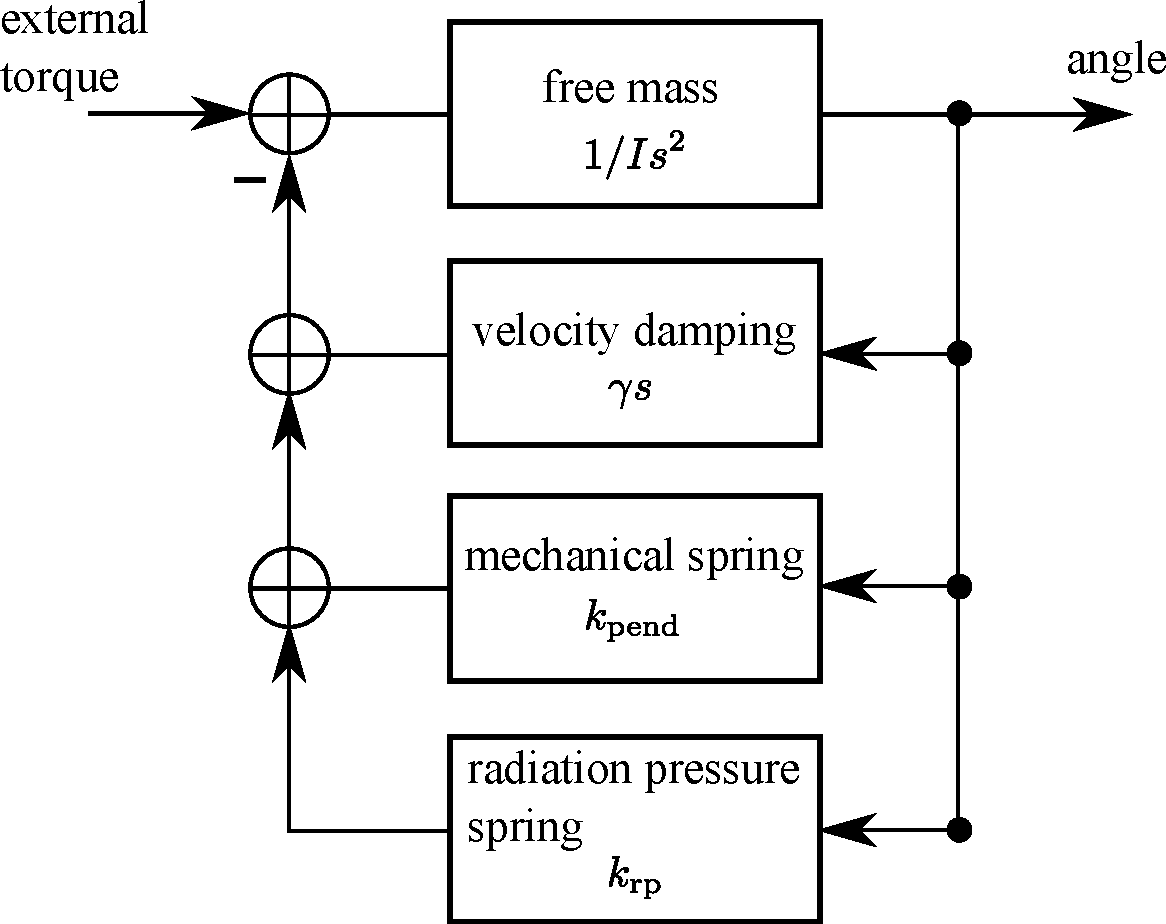
\includegraphics[width=0.6\textwidth]{figures/pendulumLoop.pdf}
\caption[Controls view of addition of radiation pressure to the pendulum
transfer function]{Demonstration of how radiation pressure modifies the torque to
  angle transfer function of a Fabry-P\'{e}rot cavity's eigenmodes.}
\label{fig:pendloop}
\end{centering}
\end{figure}

The magnitude and sign of the total torsional spring constant,
$\kappa_{tot} = \kappa_p + \kappa_{rp}$, conveys critical information
about the stability of the cavity and the nature of its response to
external torque. Recalling the equation of an angular spring, $\tau =
- \kappa_{tot} \theta$, a restoring torque is provided only if
$\kappa_{tot} > 0$, which is equivalent to the condition for
stability. If $\kappa_{tot} < 0$, the spring is an anti-spring,
resulting in an unstable, run-away situation. Furthermore, 
while $\kappa_{tot}$ is positive, its magnitude directly relates to
the stiffness of the spring.

The stability criteria for the coupled cavity eigenmodes 
depend on the relationship between $\kappa_p$ and $\kappa_{rp}$:
\begin{align}
\mbox{stable: } k_{tot} > 0 \implies & \frac{2 P L}{c (1-g_1 g_2)} \lambda < \kappa_p \\
\mbox{unstable: } k_{tot} < 0 \implies & \frac{2 P L}{c (1-g_1 g_2)} \lambda > \kappa_p.
\label{eq:stability}
\end{align}
The pendulum spring constant, $\kappa_p$, is always positive, so we
can conclude with certainty that the cavity eigenmode is stable as
long as the quantity on the left-hand side of Eq. \ref{eq:stability}
is negative. However, if this quantity is positive, then its magnitude
compared to $\kappa_p$ determines stability. Since $P$, $L$, and $c$
are all positive numbers and the $g$-factor is restricted to $0 < g_1g_2
< 1$ \footnote{This is the necessary condition for a two mirror
  resonator to form a stable periodic focusing
  system. \cite[p. 747]{Siegman1986Lasers}}, the sign of the left-hand
side is determined solely by that of $\lambda$. From the $g$-parameter
restriction, it can be shown that $\lambda_a$ is always positive and
that $\lambda_b$ is always negative. Therefore, the mode whose mirror
angles are described by $\vec{v}_a$ is either stable or unstable, and
the mode described by $\vec{v}_b$ will always be stable.

The precise situation for the potentially unstable mode depends on the
one non-constant variable, the circulating power $P$. There is a
critical power at which $\kappa_{rp}$ = - $\kappa_p$, and at any
greater power, instability ensues. In general, as power increases, the
total spring constant for the potentially unstable mode decreases,
creating a softer spring, and the total spring constant for the
unconditionally stable mode increases, creating a stiffer spring. Thus
arise the terms \emph{soft} and \emph{hard} to describe the two
eigenmodes that have been referred to by $\vec{v}_a$ and $\vec{v}_b$,
respectively.

\begin{figure}
\begin{centering}
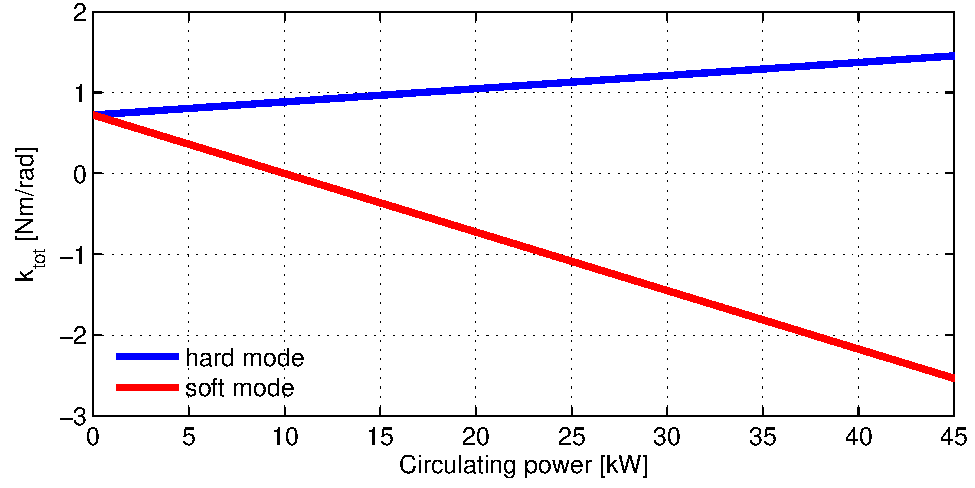
\includegraphics[width=1.0\textwidth]{figures/khardsoftLLO.pdf}
\caption[Torsional spring constants of an optically coupled
  cavity]{Torsional spring constants (pitch) of an optically coupled
  cavity for LLO parameters. The soft mode is unstable when the spring
  constant is negative.}
% Include LHO.
\label{fig:k_hardsoft}
\end{centering}
\end{figure}

Figure~\ref{fig:k_hardsoft} shows the dependence of $\kappa_{tot}$ on
circulating power for the soft and hard modes of a LIGO arm
cavity. Without power in the cavity, the modes are identical and their
spring constants are simply that of the individual pendula. The
symmetry-breaking effect of radiation pressure comes into play as soon
as light resonates in the cavity: the hard mode's spring constant
increases and the soft mode's spring constant decreases. The critical
power at which the soft mode becomes unstable is 10~kW, which
corresponds to approximately 6~W input power (for Enhanced LIGO
efficiencies) to the interferometer. Above the critical power,
radiation pressure creates an optical anti-spring. 

Table~\ref{table:k_tot} highlights the values of the spring constants
for the typical power that was used in Initial LIGO (9~kW) and for the
highest of powers achieved in Enhanced LIGO (40~kW). The corresponding
transfer functions for these spring constants is found in
Fig.~\ref{fig:optomechhardsoft}. The resonant frequency, $\omega_0 =
\sqrt{\kappa_{tot}/I}$, increases with power for the hard modes and
decreases for the soft modes. Once $\kappa_{tot}$ becomes negative, as
is the case for the Enhanced LIGO soft mode, there is no real resonant
frequency. A summary of the opto-mechanical parameters for LLO and LHO
is found in Table~\ref{table:optomech}.

\begin{table}
\centering
\caption[Torsional spring constants for the soft and hard cavity
modes]{Torsional spring constants (pitch) for the soft and hard modes
  of a typical Initial LIGO power and the highest of Enhanced LIGO
  powers. The soft mode in Enhanced LIGO is unstable. The $\kappa_p$
  values assume a resonant frequency of 0.6~Hz.}
% \textcolor{blue}{maybe include aLIGO on this table as well.}}
\begin{tabular}{l r@{ }l l r@{}l l}
\hline
 & \multicolumn{2}{l}{$P_{circ}$} & $\kappa_{p}$ & \multicolumn{2}{l}{$\kappa_{tot}$, soft mode} &
 $\kappa_{tot}$, hard mode\\
% & (kW) & (Nm/rad) & (Nm/rad) & (Nm/rad) \\
\hline
Initial LIGO & 9& kW & 0.721 Nm/rad& 0&.0734 Nm/rad & 0.867 Nm/rad\\
Enhanced LIGO & 40& kW & 0.721 Nm/rad& -2&.18 Nm/rad & 1.38 Nm/rad\\
\hline
\end{tabular}
\label{table:k_tot}
\end{table}

\begin{figure}
\begin{centering}
\subfigure{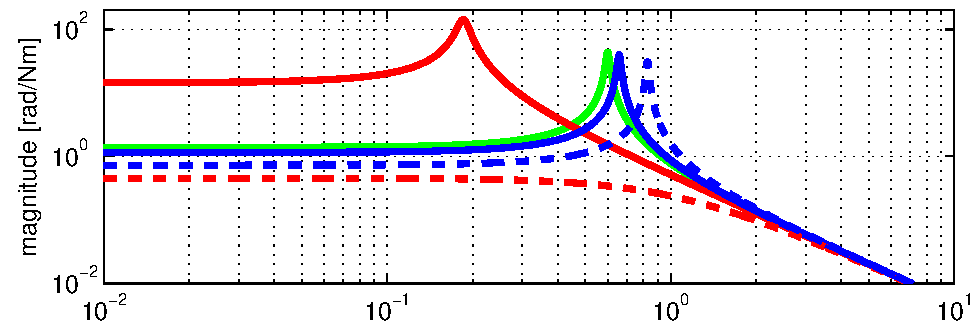
\includegraphics[width=1.0\textwidth]{figures/ieLIGOTFmags.pdf}}
\subfigure{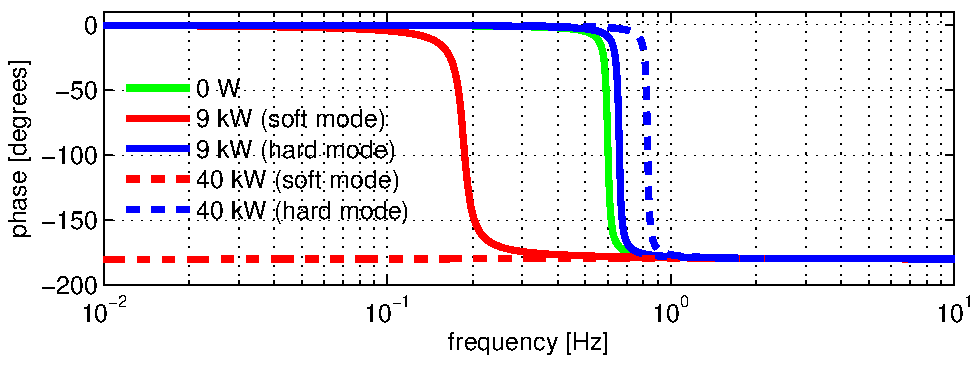
\includegraphics[width=1.0\textwidth]{figures/ieLIGOTFphases.pdf}}
\caption[Single cavity opto-mechanical transfer function]{Single
  cavity opto-mechanical transfer function for pitch. The resonant
  frequency increases with power for the hard mode, but decreases for
  the soft mode, eventually becoming imaginary. $P_{circ} = 9$ kW
  (5.25 W input) was a typical operating power for Initial LIGO and
  $P_{circ} = 40$ kW (23.5 W input) is the highest of powers reached
  for Enhanced LIGO.}
\label{fig:optomechhardsoft}
\end{centering}
\end{figure}



\begin{table}
\centering
\caption[Opto-mechanical parameters for the LIGO Livingston and LIGO
Hanford cavities]{Opto-mechanical parameters for the LIGO Livingston and LIGO
  Hanford cavities. Differences result because the mirrors at each site have different
  radii of curvature.}
\begin{tabular}{l l l l}
\hline
parameter & label & LLO & LHO \\
\hline
ITM $g$-factor & $g_1$ & 0.73 & 0.71 \\
ETM $g$-factor & $g_2$ & 0.54 & 0.45 \\
arm length & $L$ & 3995 m & 3995 m \\
test mass moment of inertia & $I$ & 0.0507 kg m$^2$ &  0.0507 kg m$^2$ \\
pendulum torsion constant & $\kappa_p$ & 0.72 Nm/rad (pitch)& 0.72 Nm/rad (pitch) \\ 
& & 0.50 Nm/rad (yaw) & 0.50 Nm/rad (yaw) \\
soft mode eigenvector & $\vec{v}_a$ & (1, 1.10) & (1, 1.14) \\
hard mode eigenvector & $\vec{v}_b$ & (-1.10, 1) & (-1.14, 1) \\
power when soft mode is unstable & $P_{crit}$ & 10.0 kW (pitch) & 11.6 kW (pitch)\\
& & 7.0 kW (yaw) & 8.0 kW (yaw) \\
\hline
\end{tabular}
\label{table:optomech}
\end{table}


\subsection{Pole Analysis}
One final comment about the analysis of the modified transfer function
(Eq. \ref{eq:modalTF}) is that the two poles,
\begin{equation}
s = s_\pm = \frac{-\gamma \pm \sqrt{\gamma^2 - 4 I \kappa_{tot}}}{2 I},
\label{eq:TFpoles}
\end{equation}
provide an alternative way to view the stability of the system. As
long as the poles are negative, the impulse response will decay or be
sinusoidal. However, if a pole is positive, the system's motion will
experience exponential growth. The constraints for $s_\pm$ to be in a
particular half of the s-plane are easily derived from
Eq. \ref{eq:TFpoles}. Note that $s_-$ will always be in the left half
of the plane and that $s_+$ is the pole that has the potential of
falling in the right half of the plane. Table \ref{table:s_0} show how
the s-plane locations for $s_+$ depend on $\kappa_{tot}$. The sign of
$\kappa_{tot}$ determines stability, as expected, and we see that the
nature of the stable response depends on the damping
coefficient. Figure \ref{fig:TFrainbow_poles} plots the pole locations
for a range of $\kappa_{tot}$ experienced while powering up Enhanced
LIGO.

% \begin{figure}
% \begin{centering}
% \subfigure{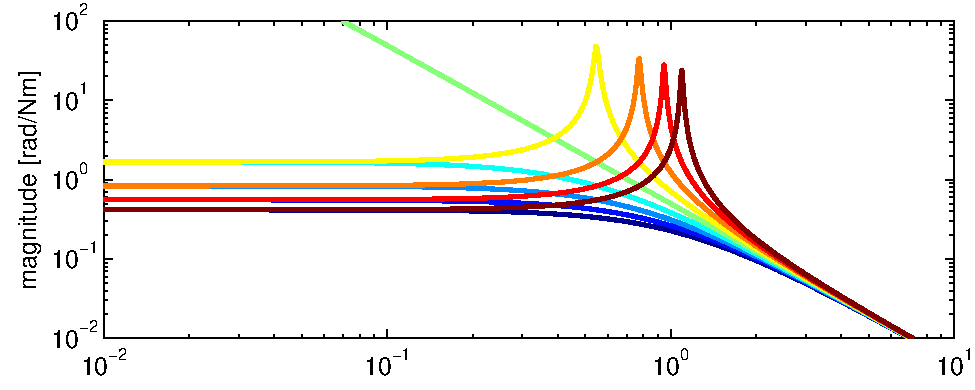
\includegraphics[width=1.0\textwidth]{figures/TFrainbow_mags.pdf}}
% \subfigure{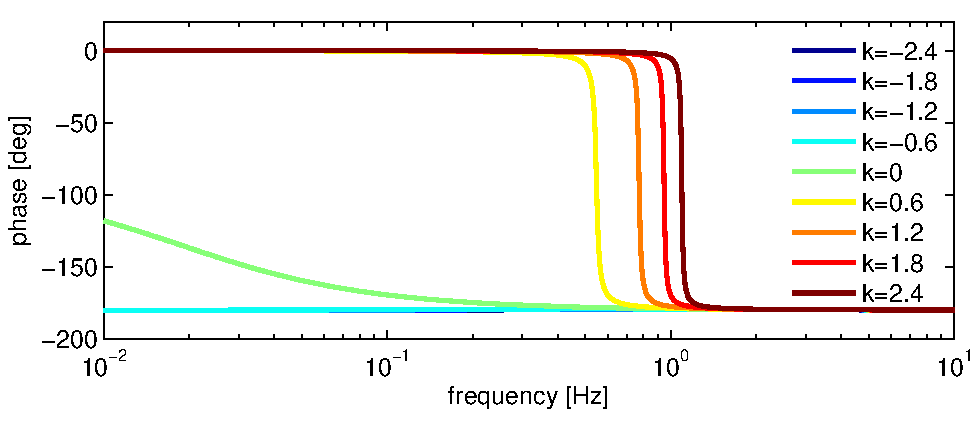
\includegraphics[width=1.0\textwidth]{figures/TFrainbow_phases.pdf}}
% \caption{Magnitude and phase of the torque to pitch transfer function
%   as a function of torsional constant for a fixed damping coefficient
%   of $\gamma^2/4I = 1.77 \times 10^{-4}$. This range of $\kappa$
%   represents the torsional constants experienced while powering up
%   Enhanced LIGO.}
% \label{fig:TFrainbow}
% \end{centering}
% \end{figure}

\begin{table}
\centering
\caption[Conditions on total torsional constant for determining system
stability]{Conditions on total torsional constant $\kappa_{tot}$ for
  determining system stability.}
\begin{tabular}{l l l}
\hline
$\kappa_{tot}$ condition & pole $s_+$ & impulse response \\
\hline
$\kappa_{tot} < 0$ & real positive & statically unstable\\
$\kappa_{tot} = 0$ & zero & \\
$0 < \kappa_{tot} < \gamma^2/4I $ & real negative & stable decay \\
$\kappa_{tot} > \gamma^2/4I$ & real negative, and imaginary & stable,
oscillatory \\
\hline
\end{tabular}
\label{table:s_0}
\end{table}


\begin{figure}
\begin{centering}
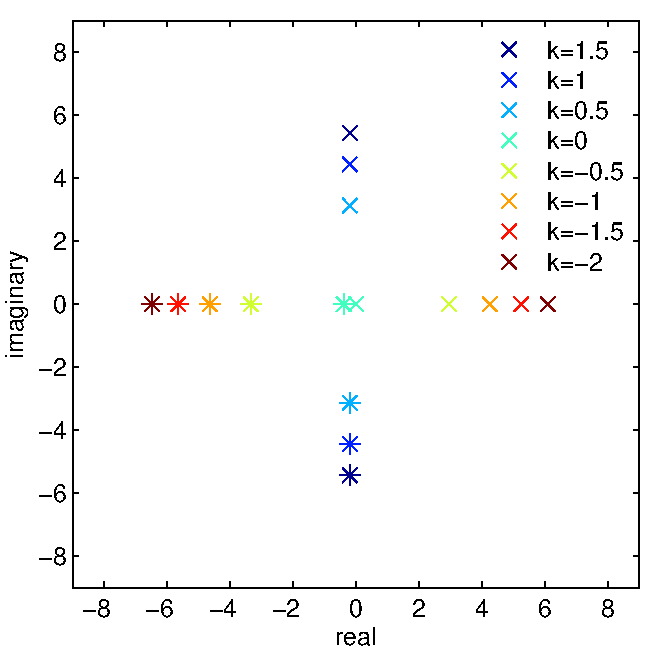
\includegraphics[width=0.667\textwidth]{figures/TFrainbow_poles.pdf}
\caption[Poles of the torque to pitch opto-mechanical transfer
function]{Poles of the torque to pitch transfer function as a function
  of torsional constant, $\kappa_{tot}$. Crosses show $s_+$ and
  asterisks show $s_-$. Poles in the right half of the s-plane
  indicate the system is unstable.}
\label{fig:TFrainbow_poles}
\end{centering}
\end{figure}







\section{Implications}
The Enhanced LIGO goal of increasing the input power to 30 W from the
Initial LIGO 7 W makes radiation pressure torques cross into the realm
of significance. In particular, the soft opto-mechanical mode which
just approached instability for Initial LIGO powers actually becomes
unstable for Enhanced LIGO powers. The transfer functions for which
controls must be designed are no longer those of a pendulum with
resonance at 0.6~Hz (pitch) or 0.5~Hz (yaw), but those of the soft and
hard eigenmodes, whose resonances change with power. For Enhanced
LIGO, the angular control servo plant of
Fig.~\ref{fig:ASCcontrolservo} is treated as the cavity's radiation
pressure-modified torque to angle transfer function, not as a simple
stand-alone pendulum transfer function. An elegant implication of the
purely geometric description of the cavity axis is that the radiation
pressure eigenmodes are orthogonal independently of power. Therefore,
the modes remain independent and the control system need not be
updated with power changes.

%\textcolor{blue}{put this elsewhere?} 
One complication of having a radiation pressure modified and therefore
power dependent plant, $P_{rp}$, is that the optical lever
compensation (described in Sec. \ref{sec:oplevcomp}) is no longer
valid. The compensation of $1+OP$ is hard-coded in the digital control
system, where the model for $P$ is that of a simple pendulum. The only
way to achieve perfect compensation would be to load a new model of
$P$ into the compensation filter bank for each new power and for each
optic. Doing this in Enhanced LIGO was not practical, so only at low
powers does the optical lever compensation actually cancel out the
effect of the optical-lever-controlled radiation pressure-modified
plant, $P_{rp}/1+OP_{rp}$, and leave simply $P_{rp}$ for the WFS to
control. It this turns out that as power increases, the imperfect
compensation actually make the loops more stable
\cite{Barsotti2008}.

The sensors in Initial LIGO were not tuned to specifically look for
the combined mirror motions that create the soft and hard modes. The
only way to provide adequate control for both modes would be to
increase the gain of all of the angular control loops. Because some of
the sensors are not as good as others, this would result in excessive
impression of sensor noise on DARM. To minimize impact on strain
sensitivity while reducing the angular motion of the interferometer's
mirrors to the levels necessary for stable operation, we need to pick
out the combination of sensors that together sense specifically the
hard mode or the soft mode, and then design controls that specifically
address the characteristics of just one mode. This is the foundation
of the ASC work for Enhanced LIGO: switching the WFS control to the
radiation pressure eigenmode basis, and increasing the gains of only
those loops that require it. 
%\textcolor{blue}{I need to make sure this is accurate.}




%\subsection{WFS Control Basis for Enhanced LIGO}